In order to verify experimental results, we also performed analyses on two real-world data sets. The
Coauthor network contains data about statistician coauthorship in prominent journals, while the
email-Eu-Core data set shows email communications within a large research institution. The data sets
were picked based upon their relatively small sizes and easy interpretability. In both cases,
vertices represent humans, which was done in order to test DSD's performance outside of the
biological domain.


\section{Selected datasets}

\subsection{Coauthor}

The Coauthor data set consist of data collected from four leading statistical journals: The Annals
of Statistics, Biometrika, the Journal of the American Statistical Association, and the Journal of
the Royal Statistical Society. Ji and Jin collected data about all papers published from 2003
through the first half of 2013 and resolved data hygiene issues such as having multiple different
published names for the same author. A graph was then constructed where every vertex corresponded to
a statistician, and edges were inserted to connect any pair of statisticians who had appeared as
coauthors. This graph was then used to cluster the authors into three statistical subdisciplines
using a spectral clustering algorithm, SCORE. The labels generated by SCORE showed a high degree of
agreement with other clustering approaches and were found to be reasonable by human researchers, so
we believe they are suitable for use as ground truth labels in a classification experiment
~\cite{ji2016}. The three labels identified were ``Objective Bayes,'' ``Biostatistics,'' and
``High-Dimensional Data Analsysis.''

After restricting to the largest connected component, the network has 4388 edges on 2263 vertices,
and so is a relatively sparse graph. It nonetheless clearly displays a scale-free degree
distribution, as can be seen from figure \ref{fig:real_world_degree_dist}.

\begin{figure}
  \centering
  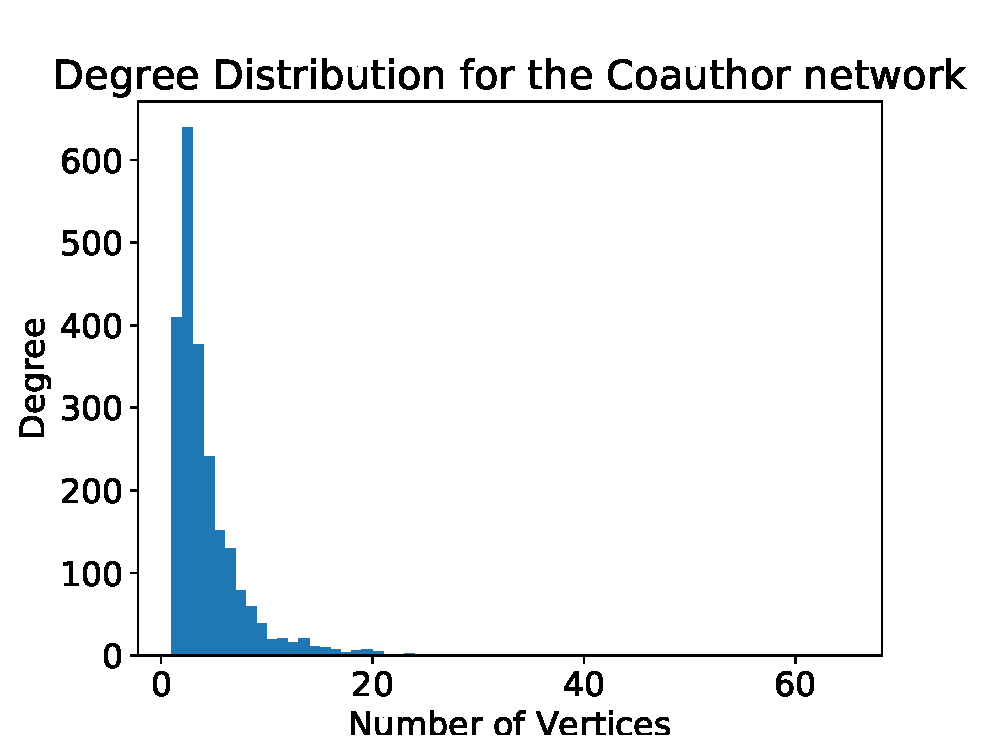
\includegraphics[width=0.48\textwidth]{coauthor_degree_dist.eps}
  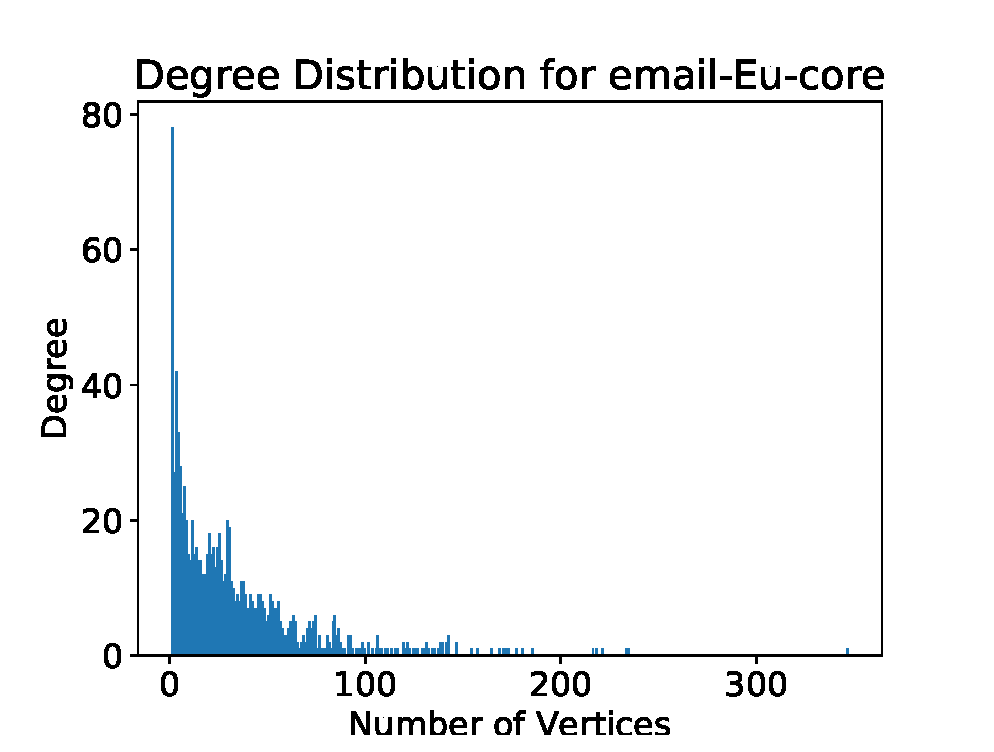
\includegraphics[width=0.48\textwidth]{email_degree_dist.eps}
  \caption{The degree distribution plots for both networks appear to show scale-free distributions}
  \label{fig:real_world_degree_dist}
\end{figure}


\subsection{email-Eu-core}

The email-Eu-core data set is built from email data collected over the course of 18 months from 2003
to 2005 at a European research institution. Each vertex corresponds to an employee at the
institution, and is labeled an integer indicating that person's department. There are a total of 48
departments in the data set. An edge was drawn between any two parties which exchanged an email over
the time period in question ~\cite{snapnets}. The original version of this data set was directed,
but we discard edge direction information for our analysis.

This graph has 986 vertices and 25571 edges after reducing to the largest connected component.
Compared to the Coauthor network, this graph is somewhat smaller and substantially denser, which
makes it an attractive candidate for demonstrating the efficacy of DSD, as such a graph would be
expected to have more and higher degree hubs than a less dense one.

In addition and in spite of its small size, this graph has 48 possible labels, indicating an average
class size of just $20.54$ elements. This means that we also have to be more conservative in
censoring data on this graph, as it would be easy to censor too high a proportion of one of the
smaller classes to be able to accurately recover the labels.


\section{Results and Analysis}

In order to evaluate the efficacy of each classifier, the label prediction experiment was done using
5-fold cross-validation on each classifier. $k=20$ was used as the parameter for the
nearest-neighbor algorithm. The results are summarized in the bar plot in figure
\ref{fig:real_world_results}.

\begin{figure}[H]
  \centering
  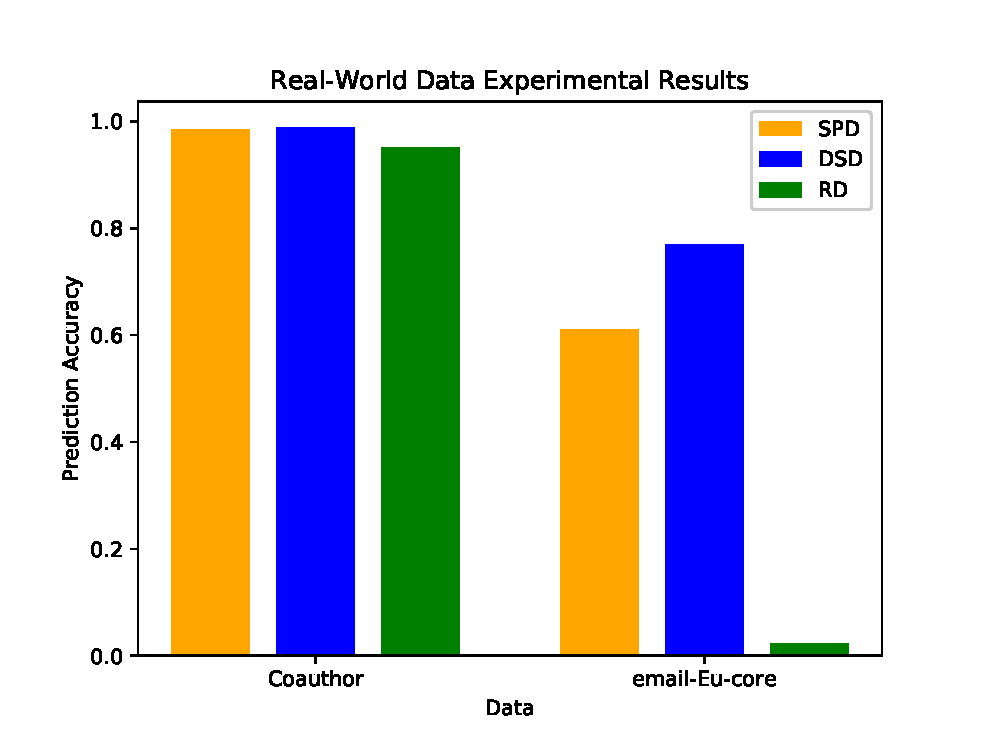
\includegraphics[width=\textwidth]{real_world_results.eps}
  \caption{Real-world data prediction accuracy results}
  \label{fig:real_world_results}
\end{figure}

The coauthor results are especially striking, as all three metrics, including resistance distance,
performed extremely well. This could probably be explained, at least partially, by the fact that the
coauthor network is fairly sparse and that the number of labels is small. However, it seems likely
that this is mostly due to the fact that SCORE was used to generate ground truth. For some reason,
the SCORE communities are clustered extremely tightly irrespective of the metric. This is an
interesting finding in its own right because it suggests that the way that we think about clusters,
at least in the context spectral clustering, probably doesn't capture some important properties of
the communities found in real-world data. The fact that resistance distance works well on the
spectral clusters but not the real ground truth is especially noteworthy in this regard.

By contrast, the email-Eu-core results are much less surprising. DSD clearly provides the dominant
classification algorithm, followed by a surprisingly strong showing from SPD. RD performs like
random guesses, as it did with most of the simulated data (recall that as there are 48 classes,
uniform random guessing would yield an expected success rate of $1/48$, or about $2.1\%$).

These results suggest that DSD has some sort of built-in model of community structure which agrees
with the real-world data. We expect that these results would generalize to work well with a wide
variety of network structures, but particularly those whose topology represents some sort of
information exchange.


%%% Local Variables:
%%% mode: latex
%%% TeX-master: "../Main"
%%% End:
